\documentclass[11pt]{article}
\input{../_estilo.tex}
\renewcommand{\tituloejercicio}{Tema 1 --- Ejercicio 14}

\begin{document}

{\LARGE\bfseries\color{azultitulo} Ejercicio 14 --- Ciclo completo: mínimo local de un arreglo}

\vspace{2pt}
\textbf{Dificultad:} $\bigstar\bigstar\bigstar$ \quad \textbf{Conferencias:} C2 a C5
\vspace{8pt}
\hrule
\vspace{12pt}

\section*{Enunciado y alcance}

\begin{enunciado}
Escoge un problema nuevo, recorre el ciclo completo de C2 y consigue que el algoritmo y la cota mínima
coincidan.
\end{enunciado}

El problema principal será encontrar un mínimo local de un arreglo de reales sin ordenar. Al final se
extiende el resultado a varias consultas. El caso central queda resuelto de forma óptima; para consultas
solapadas se dan solamente cotas.

\section{¿Cuál es el problema?}

Sea $A[0..n-1]$ un arreglo de $n\ge 1$ números reales. Se debe devolver un índice $i$ tal que

\[
(i=0\ \text{o}\ A[i-1]\ge A[i])
\quad\text{y}\quad
(i=n-1\ \text{o}\ A[i+1]\ge A[i]).
\]

Es decir, $A[i]$ no tiene un vecino menor. En los extremos se supone un centinela $+\infty$. Los valores
repetidos están permitidos; por eso se usa $\ge$ y no $>$.

Siempre existe una respuesta: un mínimo global también es un mínimo local. No se pide encontrar el mínimo
global, porque eso requiere $n-1$ comparaciones.

\subsection*{Modelo de costo}

Se trabaja en el modelo de comparaciones de C5: el algoritmo solo aprende sobre los valores mediante
comparaciones entre elementos. Cada comparación cuesta uno; índices, ciclos y aritmética son gratuitos.
Las comparaciones con $+\infty$ se resuelven por el índice y no cuentan.

\begin{resultado}{Resultado central}
Existe un algoritmo que encuentra un mínimo local con exactamente $\lceil\log_2 n\rceil$ comparaciones
en el peor caso, y ningún algoritmo del modelo puede hacerlo con menos.
\end{resultado}

La demostración sigue las cinco preguntas de C2. Primero se presenta una solución inicial, luego se obtiene
la cota mínima y finalmente se repite el ciclo para cerrar el factor que queda entre ambas.

\section{Primera ronda}

\subsection{Una solución directa}

La fuerza bruta recorre los pares consecutivos y devuelve el primer $i$ para el que $A[i]\le A[i+1]$;
si no encuentra ninguno, devuelve $n-1$.

Si devuelve un índice interior, todos los pares anteriores fueron estrictamente decrecientes, de modo que
$A[i-1]>A[i]$; además, la comparación actual da $A[i]\le A[i+1]$. En un extremo, la condición del
centinela es automática. Por tanto, el algoritmo es correcto y cuesta a lo sumo $n-1$ comparaciones.

\subsection{V1: búsqueda binaria mirando dos vecinos}

El barrido sugiere mirar solo vecinos, pero todavía los mira de izquierda a derecha. Para saltar hacia la
mitad hay que justificar que una mitad descartada no contiene todas las respuestas posibles. La observación
clave es mantener una ventana $[\mathrm{lo},\mathrm{hi}]$ con respaldo en sus dos bordes:

\[
(\mathrm{lo}=0\ \text{o}\ A[\mathrm{lo}-1]\ge A[\mathrm{lo}])
\quad\text{y}\quad
(\mathrm{hi}=n-1\ \text{o}\ A[\mathrm{hi}+1]\ge A[\mathrm{hi}]).
\]

Una ventana con respaldo contiene un mínimo local: el mínimo de la ventana no tiene un vecino menor dentro
de ella y el respaldo protege los bordes.

Por ejemplo, en la ventana $[3,7]$ del arreglo de prueba se cumple $A[2]\ge A[3]$ y
$A[8]\ge A[7]$. La ventana no necesita estar ordenada: solo importa que no se pueda salir de ella bajando.

\begin{figure}[ht]
\centering
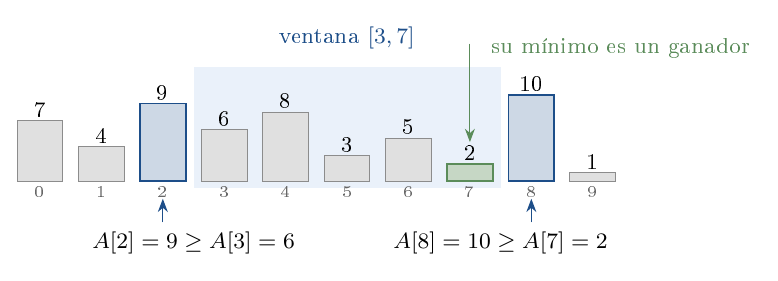
\includegraphics[width=0.92\linewidth]{images/figura-05-respaldo.png}
\caption{Una ventana con respaldo contiene un mínimo local. Los vecinos exteriores de $[3,7]$ son mayores
o iguales que sus bordes.}
\end{figure}

\begin{lstlisting}[style=pseudo]
V1(A):
    lo <- 0; hi <- n - 1
    mientras verdadero:
        m <- (lo + hi) div 2
        si m > 0 y A[m] > A[m-1]:
            hi <- m - 1
        sino si m < n-1 y A[m] > A[m+1]:
            lo <- m + 1
        sino:
            devolver m
\end{lstlisting}

\textbf{Correctitud.} El invariante es que la ventana es no vacía y tiene respaldo.

\begin{itemize}[leftmargin=18pt]
\item Al inicio, $[0,n-1]$ tiene respaldo por los centinelas.
\item Si $A[m]>A[m-1]$, entonces $m>\mathrm{lo}$. Si $m=\mathrm{lo}>0$, el respaldo izquierdo daría
      $A[m-1]\ge A[m]$, contradicción. Luego $[\mathrm{lo},m-1]$ no es vacía, conserva el borde
      izquierdo y tiene respaldo derecho porque $A[m]>A[m-1]$.
\item El caso $A[m]>A[m+1]$ es simétrico: $m<\mathrm{hi}$ y la ventana $[m+1,\mathrm{hi}]$ conserva
      el respaldo.
\item Si ninguna rama se toma, $m$ no tiene vecino menor y se devuelve una respuesta correcta.
\end{itemize}

Esta es la idea que permite descartar media ventana. Si $A[m-1]<A[m]$, se conserva la mitad izquierda y
$A[m]$ se convierte en el nuevo respaldo derecho. Si $A[m+1]<A[m]$, se conserva la mitad derecha y $A[m]$
se convierte en el nuevo respaldo izquierdo.

\begin{figure}[ht]
\centering
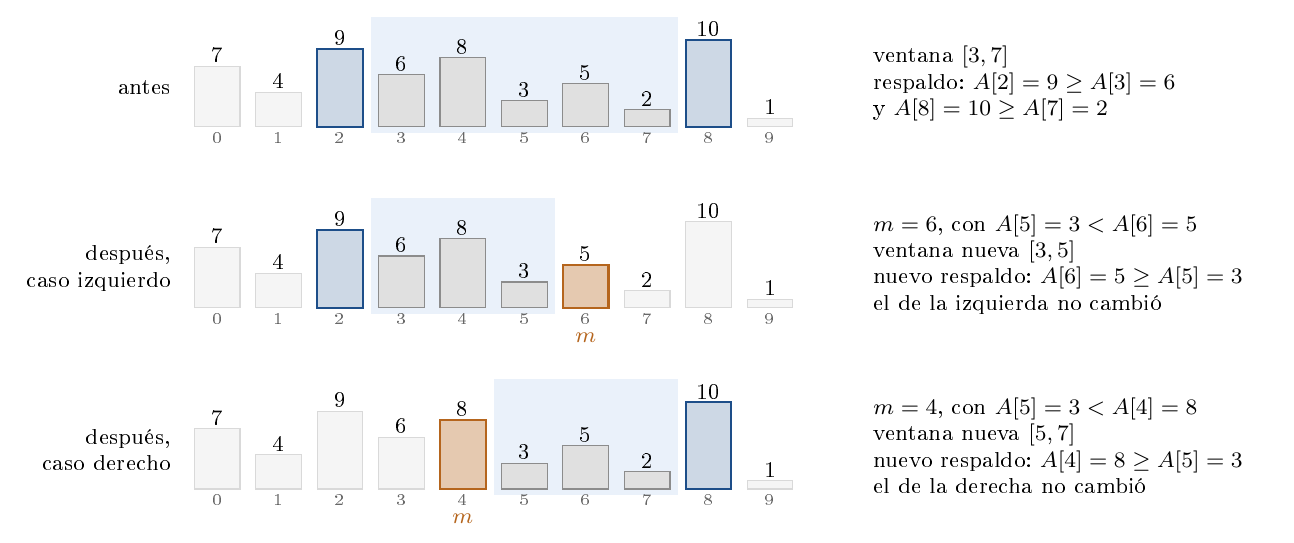
\includegraphics[width=\linewidth]{images/figura-07-achica.png}
\caption{Las dos formas de achicar una ventana con respaldo. El nuevo borde queda protegido por el elemento
$m$ que se acaba de comparar.}
\end{figure}

Para la terminación, el potencial $D=\mathrm{hi}-\mathrm{lo}$ es un natural y disminuye estrictamente
en cada rama. V1 es, por tanto, totalmente correcto.

La ventana se reduce a lo sumo a la mitad en cada vuelta, pero se hacen hasta dos comparaciones:

\[
\text{costo de V1}\le 2\lfloor\log_2 n\rfloor+2=O(\log n).
\]

La primera ronda produce una solución logarítmica, pero todavía no demuestra optimalidad.

\section{¿Se puede hacer mejor? Cota mínima}

Para cada $k\in\{0,\dots,n-1\}$ consideremos

\[
V_k[i]=
\begin{cases}
2(k-i), & i<k,\\
0, & i=k,\\
2(i-k)-1, & i>k.
\end{cases}
\]

El arreglo decrece estrictamente hasta $k$ y crece estrictamente después.

\begin{figure}[ht]
\centering
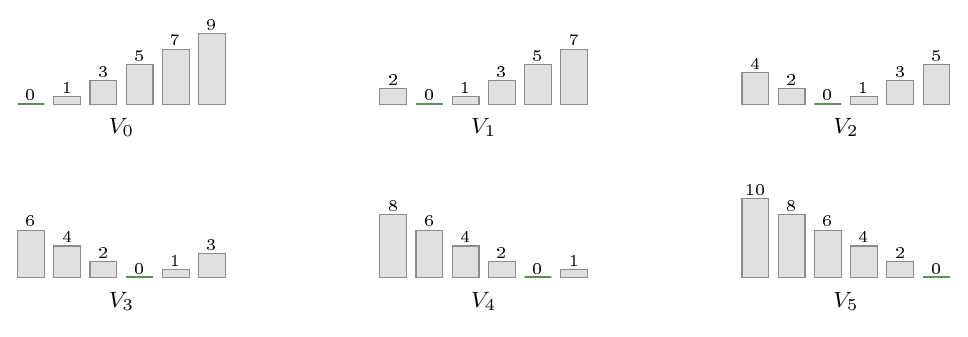
\includegraphics[width=\linewidth]{images/figura-10-vk.png}
\caption{Cada $V_k$ tiene su único mínimo local en la posición $k$. Estas instancias fuerzan respuestas
distintas en el árbol de decisión.}
\end{figure}

\begin{resultado}{Lema: respuesta única}
$k$ es el único mínimo local de $V_k$.
\end{resultado}

\textbf{Demostración.} Si $i<k$, entonces $V_k[i]>V_k[i+1]$, de modo que $i$ no es mínimo local.
Si $i>k$, entonces $V_k[i-1]<V_k[i]$, y tampoco lo es. En $k$, el valor es menor que sus vecinos,
incluidos los centinelas si corresponde. $\square$

Consideremos el árbol de decisión de cualquier algoritmo correcto. La salida depende únicamente de la hoja:
dos entradas que siguen el mismo camino reciben las mismas respuestas y producen la misma salida. Como
$V_k$ y $V_{k'}$ tienen respuestas únicas y distintas cuando $k\ne k'$, deben llegar a hojas distintas.

En los arreglos $V_k$ todos los valores son distintos, por lo que solo se usan dos ramas de cada
comparación. El árbol tiene al menos $n$ hojas. Si su altura es $h$, entonces

\[
2^h\ge n,
\qquad\text{luego}\qquad
h\ge\lceil\log_2 n\rceil.
\]

Así, todo algoritmo de comparaciones necesita al menos $\lceil\log_2 n\rceil$ comparaciones en el peor
caso.

\section{Segunda ronda: V2}

V1 compara a $m$ con dos vecinos. Para elegir una mitad solo hace falta una comparación. Definamos

\[
P(i)=[A[i]>A[i+1]],\qquad i=0,\dots,n-2,
\]

y además $P(-1)=\text{cierto}$ y $P(n-1)=\text{falso}$. La sucesión comienza en cierto y termina en
falso, así que tiene una transición cierto--falso. Si ocurre entre $i-1$ e $i$, entonces
$A[i-1]>A[i]\le A[i+1]$ y $i$ es un mínimo local.

La sucesión $P$ convierte el problema en encontrar una transición: mientras $P(i)$ es cierto, el arreglo
baja hacia la derecha; cuando pasa a falso, aparece un mínimo local. V2 busca esa transición, no un elemento
en un arreglo ordenado.

\begin{lstlisting}[style=pseudo]
V2(A):
    lo <- 0; hi <- n - 1
    mientras lo < hi:
        m <- (lo + hi) div 2
        si A[m] > A[m+1]:
            lo <- m + 1
        sino:
            hi <- m
    devolver lo
\end{lstlisting}

\begin{figure}[ht]
\centering
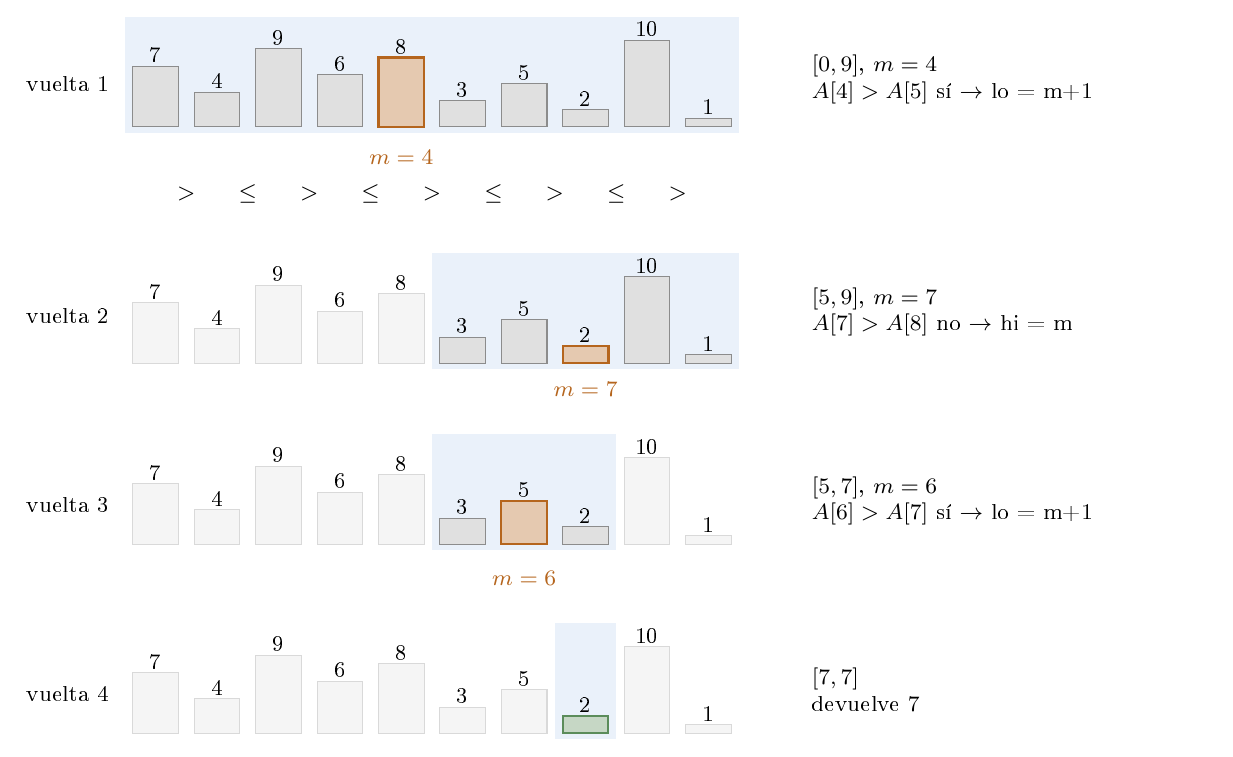
\includegraphics[width=0.78\linewidth]{images/figura-12-v2.png}
\caption{V2 sobre $[7,4,9,6,8,3,5,2,10,1]$. Cada vuelta conserva la transición cierto--falso y hace una
sola comparación.}
\end{figure}

\subsection*{Correctitud}

El invariante, al evaluar la guarda, es

\[
0\le\mathrm{lo}\le\mathrm{hi}\le n-1,
\qquad P(\mathrm{lo}-1)=\text{cierto},
\qquad P(\mathrm{hi})=\text{falso}.
\]

\textbf{Inicialización.} Para $\mathrm{lo}=0$, $P(-1)$ es cierto por el centinela izquierdo. Para
$\mathrm{hi}=n-1$, $P(n-1)$ es falso por el centinela derecho.

\textbf{Mantenimiento.} Si $P(m)$ es cierto, se asigna $\mathrm{lo}'=m+1$; entonces
$P(\mathrm{lo}'-1)=P(m)$ sigue siendo cierto y el límite derecho no cambia. Si $P(m)$ es falso, se
asigna $\mathrm{hi}'=m$; entonces $P(\mathrm{hi}')=P(m)$ sigue siendo falso y el límite izquierdo no
cambia. En ambos casos el invariante se conserva.

\textbf{Conclusión.} Al salir, $\mathrm{lo}=\mathrm{hi}=i$. El invariante da $P(i-1)$ cierto y $P(i)$
falso, es decir, $A[i-1]>A[i]\le A[i+1]$. Por tanto, $i$ es un mínimo local.

\textbf{Terminación.} Si $P(m)$ es cierto, $\mathrm{lo}$ aumenta; si es falso, $\mathrm{hi}$ disminuye.
En ambos casos el potencial $\mathrm{hi}-\mathrm{lo}$ disminuye estrictamente. V2 termina y es correcto.

\subsection*{Costo}

Cada vuelta hace una sola comparación. Si la ventana tiene tamaño $s$, la nueva ventana tiene tamaño a lo
sumo $\lceil s/2\rceil$. Después de $t$ comparaciones su tamaño es a lo sumo $\lceil n/2^t\rceil$,
de modo que termina cuando $2^t\ge n$. Por tanto,

\[
\text{costo de V2}\le\lceil\log_2 n\rceil.
\]

La cota mínima anterior da la desigualdad contraria para cualquier algoritmo.

\begin{resultado}{Algoritmo y cota coinciden}
V2 es óptimo: su costo en el peor caso es exactamente $\lceil\log_2 n\rceil$ comparaciones.
Para una consulta de longitud $L$, el costo óptimo es $\lceil\log_2 L\rceil$.
\end{resultado}

\begin{figure}[ht]
\centering
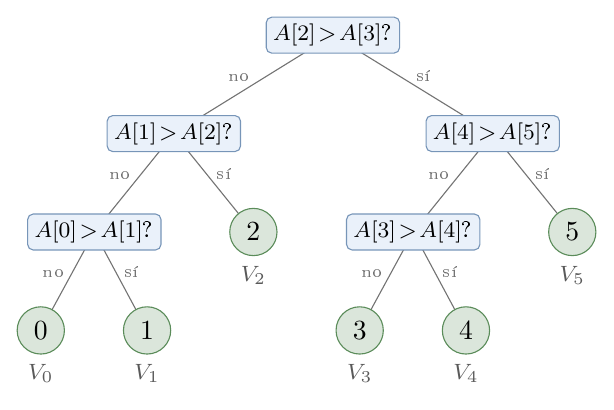
\includegraphics[width=0.58\linewidth]{images/figura-13-arbol.png}
\caption{Para $n=6$, el árbol de V2 tiene seis hojas, una por posible posición de la transición, y altura
$\lceil\log_2 6\rceil=3$.}
\end{figure}

\section{Extensión: varias consultas}

Consideremos consultas $(l_j,r_j)$ de longitudes $L_j=r_j-l_j+1$. Cada consulta es un arreglo independiente
con $+\infty$ en sus dos bordes. V2 se aplica a esa vista y el índice local se desplaza por $l_j$.

Si se recuerdan las comparaciones, solo se almacenan pares adyacentes $(m,m+1)$ de $A$. Para consultas
arbitrarias,

\[
\text{costo de V2 con memoria}
\le
\min\left(n-1,\sum_j\lceil\log_2 L_j\rceil\right).
\]

La primera cota cuenta los pares adyacentes posibles de todo el arreglo; la segunda suma el costo máximo
de cada consulta por separado.

\subsection*{Consultas disjuntas}

Si los rangos son disjuntos dos a dos, la suma es también una cota mínima. En cada rango $j$ se coloca
una instancia $V_{k_j}$ y se elige una constante $M$ suficientemente grande para que los valores de
bloques distintos estén separados. Las comparaciones entre rangos no revelan nada sobre los índices
$k_j$.

El adversario mantiene un conjunto $C_j$ de posiciones todavía posibles. Una comparación interna divide
$C_j$ según su resultado y el adversario conserva la parte más grande. Después de $t_j$ comparaciones
quedan al menos

\[
\left\lceil\frac{L_j}{2^{t_j}}\right\rceil
\]

posibilidades. Si $t_j<\lceil\log_2L_j\rceil$, quedan dos instancias con el mismo historial de respuestas
pero con respuestas correctas distintas. El algoritmo fallaría en una de ellas. Así,

\[
\mathrm{OPT}\ge\sum_j\lceil\log_2L_j\rceil.
\]

Junto con la cota superior, V2 es exactamente óptimo para consultas disjuntas.

\subsection*{Consultas solapadas}

Para consultas solapadas queda demostrado

\[
\max_{S\subseteq Q\ \text{disjunta}}
\sum_{j\in S}\lceil\log_2L_j\rceil
\le \mathrm{OPT}(Q)\le
\min\left(n-1,\sum_j\lceil\log_2L_j\rceil\right).
\]

Estas cotas no siempre coinciden. Por ejemplo, para $n=4$ y $Q=\{(0,2),(1,3)\}$ existe un algoritmo de
dos comparaciones, mientras que aplicar V2 a cada consulta y recordar resultados puede usar tres. Este
caso queda como extensión acotada, no como parte del resultado óptimo principal.

\section*{Conclusión}

El problema central queda completamente resuelto:

\begin{enumerate}[leftmargin=22pt]
\item La fuerza bruta cuesta $n-1$ comparaciones.
\item V1 reduce el costo a $O(\log n)$, pero usa hasta dos comparaciones por vuelta.
\item La familia $V_k$ demuestra la cota mínima $\lceil\log_2n\rceil$.
\item V2 hace una comparación por vuelta y alcanza exactamente esa cota.
\end{enumerate}

Para consultas disjuntas, el costo óptimo es la suma de las cotas individuales. Para consultas solapadas se
obtienen las cotas anteriores, pero no una caracterización exacta en este desarrollo.

Las pruebas de \texttt{verif.py} comprueban empates, arreglos monótonos, valles, permutaciones y consultas
pequeñas. Respaldan el argumento, pero la correctitud y la optimalidad se siguen de las demostraciones.

\begin{alerta}{Errores que hay que evitar}
Confundir mínimo local con mínimo global; suponer que el arreglo está ordenado; olvidar los centinelas en
los extremos de una consulta; sumar automáticamente los costos de consultas solapadas; u omitir que la cota
vale únicamente para el modelo de comparaciones.
\end{alerta}

\end{document}
